% Dokumentacja projektu grupowego - Metody opracowywania interfejsów użytkownika
% UKEN Kraków, rok akademicki 2026/2027
%
% Kompilacja: pdflatex dokumentacja.tex (dwa razy - spis treści i numery stron)
% albo w Overleaf: wgrać cały folder jako projekt (New Project → Upload Project).
%
% Co uzupełniacie:
% 1. dane projektu poniżej (sekcja DANE PROJEKTU),
% 2. treść rozdziałów w folderze rozdzialy/,
% 3. zrzuty ekranu w folderze obrazy/ (nazwy plików jak w poleceniach \zrzut).
% Oddajecie PDF tej dokumentacji: w Zadaniach w Teams i w repozytorium (folder docs/).
% Tekst szary w nawiasach kwadratowych \wpisz{...} zastępujecie własną treścią.
% Przed oddaniem przełączcie \pokazinstrukcjetrue na \pokazinstrukcjefalse,
% żeby zniknęły szare ramki z instrukcjami.
\documentclass[11pt,a4paper]{article}
\usepackage{dokumentacja}

% WŁĄCZENIE / WYŁĄCZENIE INSTRUKCJI
% \pokazinstrukcjetrue % szablon: instrukcje widoczne
\pokazinstrukcjefalse % wersja do oddania: instrukcje ukryte

% STUDIA NIESTACJONARNE
% \niestacjonarnetrue % odkomentujcie tylko na studiach niestacjonarnych

% UCZELNIA I PRZEDMIOT (ustawione - zmieniać tylko w razie potrzeby)
% \wydzial{} % pusty - wiersz z wydziałem się nie pokazuje
% \instytut{Instytut Nauk Technicznych}
% \kierunek{Informatyka}
% \prowadzaca{mgr inż. Aleksandra Olszyńska}

% DANE PROJEKTU
\nazwaprojektu{Planer sesji i terminów}
\podtytulprojektu{Aplikacja, w której student zbiera terminy kolokwiów, egzaminów i projektów i od razu widzi, co ma najbliżej}
\tematprojektu{8. Planer sesji i terminów}
\nazwazespolu{Zespół 8}
\numerzespolu{8} % numer zespołu = numer tematu z pliku zapisów
\grupalab{LB2}
\repozytorium{\url{https://github.com/Machux133/MOIU-Planer-Sesji-I-Terminow}}
\technologia{Astro 7, React 19, TypeScript, CSS}
\wersjadokumentu{0.3 - stan na L6 (wersja robocza)}
\dataoddania{25.11.2026}

% skład zespołu: \osoba{imię i nazwisko}{nr albumu}{rola w projekcie}
\osoba{Mateusz Machowski}{179734}{ramy graficzne, start, lista i szczegóły, nawigacja, wąski ekran}
\osoba{Bartosz Kurbiel}{177909}{formularz, walidacja, dane i operacje (edycja, usuwanie)}

\hypersetup{pdftitle={Dokumentacja projektu},pdfsubject={Metody opracowywania interfejsów użytkownika}}

\begin{document}

\stronatytulowa

% metryczka, spisy
% Metryczka dokumentu (strona 2)
\section*{Metryczka dokumentu}
\addcontentsline{toc}{section}{Metryczka dokumentu}

\begin{instrukcja}[zalecane]
Historia wersji pokazuje, jak dokument powstawał. Wpiszcie co najmniej trzy wersje: koncepcję oddaną
jako K1, stan przy prototypie K2 i wersję końcową. Przed oddaniem wyłączcie instrukcje w pliku
\texttt{dokumentacja.tex} (\texttt{\textbackslash pokazinstrukcjefalse}).
\end{instrukcja}

\subsection*{Dane projektu}
\tabeladanych

\subsection*{Skład zespołu}
\tabelaskladu

\subsection*{Historia wersji}
\begin{tabularx}{\linewidth}{@{}p{1.6cm}p{2.4cm}p{3.6cm}L@{}}
\naglowektabeli \nt{Wersja} & \nt{Data} & \nt{Autor} & \nt{Opis zmian} \\
0.1 & 17.11.2026 & obie osoby & koncepcja i makiety (punkt kontrolny K1) \\
0.2 & 18.11.2026 & M. Machowski & szkielet aplikacji: Astro, ramy graficzne, nawigacja, cztery ekrany \\
0.3 & 25.11.2026 & M. Machowski & ekran startowy, lista z filtrem, szczegóły, wąski ekran; pierwsza wersja dokumentacji \\
0.4 & 25.11.2026 & B. Kurbiel & formularz, walidacja, zapis i sprawdzenie przebiegu dodawania terminu \\
\bottomrule
\end{tabularx}
\newpage


\tableofcontents
\listoffigures
\listoftables
\newpage

% rozdziały
% 1. Wprowadzenie
\section{Wprowadzenie}\label{sec:wprowadzenie}

\begin{instrukcja}[zalecane]
Krótko: czym jest aplikacja, jaki problem rozwiązuje i co zespół zrobił w ramach projektu. Wypiszcie,
czego świadomie nie robiliście (poza zakresem) - to pokazuje, że trzymaliście się minimum z karty
projektu. Pół strony wystarczy.
\end{instrukcja}

\subsection{Cel projektu}
W sesji student ma kilkanaście terminów z różnych przedmiotów rozrzuconych po wiadomościach,
kalendarzach i notatkach. Planer zbiera je w jednym miejscu, na starcie pokazuje najbliższy termin
z liczbą dni do niego, a na liście wyróżnia terminy pilne. Dzięki temu student szybko sprawdza,
co ma najbliżej i jaki materiał obowiązuje.

\subsection{Zakres projektu}
Zakres minimalny z karty projektu i jego realizacja:

\begin{table}[H]\centering
\caption{Realizacja zakresu minimalnego}\label{tab:zakres}
\begin{tabularx}{\linewidth}{@{}p{0.6cm}p{5.4cm}p{2.6cm}L@{}}
\naglowektabeli \nt{\#} & \nt{Element zakresu} & \nt{Stan} & \nt{Gdzie w aplikacji} \\
1 & ekran startowy & \tak & Start (\texttt{/}) \\
2 & lista elementów & \tak & Terminy (\texttt{/terminy}) \\
3 & ekran szczegółów & \tak & Szczegóły (\texttt{/termin?id=}) i panel obok listy \\
4 & formularz z walidacją & \czesciowo & Dodaj termin (\texttt{/dodaj}); reguły w \texttt{validate.ts}, formularz w budowie \\
5 & nawigacja łącząca co najmniej 4 ekrany & \tak & stałe menu: Start, Terminy, Dodaj termin; okruszki \\
6 & wersja na wąski ekran & \tak & dolny pasek nawigacji, jedna kolumna (rozdział \ref{sec:waski}) \\
\bottomrule
\end{tabularx}
\end{table}

\textbf{Poza zakresem} (świadomie pominięte): konta i logowanie, synchronizacja między urządzeniami, serwer, wysyłanie powiadomień (przypomnienie jest tylko zapisywane przy terminie), import z USOS.

% 2. Użytkownik i cel
\section{Użytkownik i cel}\label{sec:uzytkownik}

\begin{instrukcja}[wymagane]
Kto korzysta z aplikacji, w jakiej sytuacji i po co (Wykład 1). Opiszcie głównego użytkownika jako
personę, jego cel i dwa-trzy najważniejsze zadania. Odwołajcie się do pojęć z wykładu: cel użytkownika,
skala od sporadycznego do zaawansowanego, wzorce zachowań (np. Satisficing, Pragnienie Natychmiastowej
Satysfakcji).
\end{instrukcja}

\subsection{Persona}
\begin{ramka}{Kasia, 21 lat, studentka III roku informatyki}
\begin{tabularx}{\linewidth}{@{}>{\bfseries}p{3.6cm}L@{}}
Sytuacja & między zajęciami na telefonie sprawdza, co ją czeka w tym tygodniu; wieczorem przy komputerze dopisuje nowe terminy podane przez prowadzących \\
Główny cel & nie przegapić żadnego zaliczenia i wiedzieć, ile czasu zostało na naukę i jaki materiał obowiązuje \\
Doświadczenie & środek skali: korzysta kilka razy w tygodniu, zna aplikację, ale nie chce uczyć się skrótów ani ustawień \\
Frustracje & terminy są rozproszone (Teams, USOS, notatki), a ogólny kalendarz miesza zaliczenia z resztą spraw i nie pokazuje zakresu materiału \\
\end{tabularx}
\end{ramka}

\subsection{Główne zadania użytkownika}
\begin{enumerate}
  \item sprawdzić najbliższy termin i liczbę dni do niego (ekran startowy, 0 kliknięć)
  \item przejrzeć terminy jednego przedmiotu i zakres materiału (lista z filtrem, szczegóły)
  \item dopisać nowy termin podany na zajęciach (formularz „Dodaj termin”)
\end{enumerate}

\subsection{Wzorce zachowań, które uwzględniliśmy}
\textbf{Pragnienie Natychmiastowej Satysfakcji:} najważniejsza informacja (najbliższy termin i liczba
dni) jest na ekranie startowym bez żadnego kliknięcia.
\textbf{Satisficing:} użytkownik klika pierwszą rzecz, która wygląda na dobrą, dlatego cała karta
terminu jest klikalna, a polecenie główne „Dodaj termin” jest jedno i wyraźne.
\textbf{Bezpieczna Eksploracja:} stałe menu i okruszki pozwalają wrócić w każdej chwili, więc można
spokojnie zaglądać w szczegóły.

% 3. Wymagania
\section{Wymagania}\label{sec:wymagania}

\begin{instrukcja}[zalecane]
Wymagania funkcjonalne mówią, co aplikacja robi, a niefunkcjonalne - jaka ma być. Każde wymaganie ma
identyfikator (WF-1, WN-1), żeby można się do niego odwołać w testach (rozdział \ref{sec:testy}).
Priorytet: \textbf{M} - musi być, \textbf{P} - powinno być, \textbf{O} - opcjonalne.
\end{instrukcja}

\subsection{Wymagania funkcjonalne}
\begin{table}[H]\centering
\caption{Wymagania funkcjonalne}\label{tab:wf}
\begin{tabularx}{\linewidth}{@{}p{1.2cm}Lp{1.6cm}p{2.4cm}@{}}
\naglowektabeli \nt{ID} & \nt{Opis} & \nt{Priorytet} & \nt{Stan} \\
WF-1 & \wpisz{użytkownik przegląda listę ofert z podziałem na kierunki} & M & \wpisz{zrealizowane} \\
WF-2 & \wpisz{użytkownik filtruje listę po przedmiocie} & P & \\
WF-3 & \wpisz{użytkownik dodaje ofertę przez formularz z walidacją} & M & \\
WF-4 & \wpisz{...} & & \\
\bottomrule
\end{tabularx}
\end{table}

\subsection{Wymagania niefunkcjonalne}
\begin{table}[H]\centering
\caption{Wymagania niefunkcjonalne}\label{tab:wn}
\begin{tabularx}{\linewidth}{@{}p{1.2cm}Lp{4.2cm}@{}}
\naglowektabeli \nt{ID} & \nt{Opis} & \nt{Jak sprawdzone} \\
WN-1 & interfejs działa na ekranie o szerokości 360 px bez przewijania w bok & \wpisz{narzędzia deweloperskie, telefon} \\
WN-2 & kontrast tekstu co najmniej 4,5:1 & \wpisz{narzędzie do kontrastu} \\
WN-3 & wszystkie funkcje dostępne z klawiatury & \wpisz{test klawiszem Tab} \\
WN-4 & \wpisz{...} & \\
\bottomrule
\end{tabularx}
\end{table}

% 4. Architektura informacji i nawigacja
\section{Ekrany i nawigacja}\label{sec:nawigacja}

\begin{instrukcja}[wymagane]
Lista ekranów i mapa przejść między nimi. Nazwijcie model nawigacji z Wykładu 1 (np. oś i szprychy,
pełne połączenie, wiele poziomów, krok po kroku; jeden serwis może łączyć dwa modele) i uzasadnijcie go w 1-2 zdaniach. Mapę możecie zmienić w kodzie
TikZ poniżej albo zastąpić obrazkiem (\texttt{\textbackslash zrzut\{mapa\_ekranow.png\}\{...\}\{0.9\}}).
\end{instrukcja}

\subsection{Lista ekranów}
\begin{table}[H]\centering
\caption{Ekrany aplikacji}\label{tab:ekrany}
\begin{tabularx}{\linewidth}{@{}p{0.6cm}p{3.6cm}Lp{3.4cm}@{}}
\naglowektabeli \nt{\#} & \nt{Ekran} & \nt{Do czego służy} & \nt{Przejścia do} \\
E1 & Start (\texttt{/}) & najbliższy termin z liczbą dni, polecenie „Dodaj termin”, trzy następne terminy & E2, E3, E4 \\
E2 & Terminy (\texttt{/terminy}) & wszystkie terminy według daty, filtr po przedmiocie, wyróżnione pilne; na szerokim ekranie szczegóły w panelu obok & E3, E1, E4 \\
E3 & Szczegóły (\texttt{/termin?id=}) & pełne dane terminu: data, liczba dni, sala, zakres, notatki, przypomnienie & E2, E4 (edycja) \\
E4 & Dodaj / edytuj (\texttt{/dodaj}) & formularz nowego terminu albo edycji istniejącego & E2 (po zapisie) \\
\bottomrule
\end{tabularx}
\end{table}

\subsection{Mapa ekranów}
\begin{figure}[H]\centering
\begin{tikzpicture}[node distance=1.2cm and 1.6cm]
  \node[ekranglowny] (start) {E1\\Start};
  \node[ekran, right=of start] (lista) {E2\\Terminy};
  \node[ekran, right=of lista] (szcz) {E3\\Szczegóły};
  \node[ekran, below=of lista] (form) {E4\\Dodaj / edytuj};
  \draw[przejscie] (start) -- node[opis,above]{zobacz wszystkie} (lista);
  \draw[przejscie] (lista) -- node[opis,above]{wybór terminu} (szcz);
  \draw[przejscie] (start.north) -- ++(0,0.7) -| node[opis,pos=0.25,above]{karta najbliższego terminu} (szcz.north);
  \draw[przejscie] (start) |- node[opis,pos=0.75,below]{Dodaj termin} (form);
  \draw[przejscie] (szcz) |- node[opis,pos=0.75,below]{Edytuj termin} (form);
  \draw[powrot] (form) -- node[opis,right]{zapisz} (lista);
\end{tikzpicture}
\caption{Mapa ekranów i przejść; z każdego ekranu stałe menu prowadzi do E1, E2 i E4 (nie rysowane)}\label{rys:mapa}
\end{figure}

\subsection{Model nawigacji}
\textbf{Model:} wiele poziomów (płytka hierarchia, dwa poziomy) połączony ze stałą nawigacją globalną.\\
\textbf{Uzasadnienie:} student przechodzi od ogółu (lista terminów) do szczegółu (jeden termin), więc
naturalne są dwa poziomy. Trzy ekrany najwyższego poziomu są zawsze widoczne w menu, bo przy trzech
pozycjach nie ma powodu chować ich w menu rozwijanym, a „Dodaj termin” jest najczęstszą akcją zmieniającą
dane. Każdy ekran jest osiągalny w najwyżej dwóch kliknięciach.

\subsection{Orientacja użytkownika}
Aktywna pozycja menu ma wypełnione tło i atrybut \texttt{aria-current="page"}. Na ekranach poziomu 2
i w formularzu są Okruszki (Start \textgreater{} Terminy \textgreater{} Szczegóły), a na szczegółach także link
„Wróć do listy”. Każdy ekran ma własny adres, więc działa przycisk „Wstecz” przeglądarki, a stan listy
(filtr i wybrany termin) jest zapisany w adresie (\texttt{?przedmiot=\&id=}) i nie ginie po odświeżeniu.

\subsection{Ścieżka głównego zadania}
Sprawdzenie najbliższego terminu: 0 kliknięć (widać go od razu na ekranie startowym). Zakres materiału
najbliższego terminu: Start $\to$ karta najbliższego terminu (1 kliknięcie). Terminy jednego przedmiotu:
Start $\to$ Terminy $\to$ filtr przedmiotu (2 kliknięcia). Dodanie terminu: „Dodaj termin” z menu albo ze
Startu (1 kliknięcie do formularza).

% 5. Projekt interfejsu
\section{Projekt interfejsu}\label{sec:projekt}

\begin{instrukcja}[zalecane]
Pokażcie drogę od makiety do gotowego ekranu i opiszcie decyzje wizualne z Wykładu 2: Ramy Graficzne
(stałe elementy na wszystkich ekranach), hierarchię wizualną (co dominuje na ekranie) i układ.
Makiety z K1 dajcie do załącznika A, a tutaj jedno porównanie makieta - ekran końcowy.
\end{instrukcja}

\subsection{Od makiety do ekranu}
\zrzut{makieta_lista.png}{Makieta listy z punktu kontrolnego K1}{0.8}
\zrzut{e2_lista.png}{Ekran listy w obecnej wersji (szeroki ekran, dwa panele)}{0.8}
Układ z makiety został zachowany: boczne menu, filtr w postaci przycisków, lista kart po lewej
i szczegóły wybranego terminu po prawej. Szarości zastąpił jeden kolor akcentu, a znaczniki typu
dostały ikony z zestawu Lucide obok tekstu. Przyciski „Edytuj termin” i „Usuń termin” z makiety
zostaną dodane razem z formularzem (L7).

\subsection{Ramy Graficzne i hierarchia wizualna}
Ekrany mają wspólny układ (\texttt{Layout.astro}) i wspólne style
(\texttt{global.css}): to samo menu w tym samym miejscu, ten sam krój, kolory, promienie i odstępy.
Na ekranie startowym dominuje karta najbliższego terminu: jest największa, ma grubszą ramkę, cień
i liczbę dni zapisaną cyfrą wielkości 4\,rem; dodatkowo wokół ramki krąży subtelny punkt światła.
Na liście dominuje zaznaczony termin i jego panel szczegółów, a na szczegółach blok z datą i liczbą dni.
Polecenie główne „Dodaj termin” to jedyny wypełniony przycisk w kolorze akcentu, z ikoną.

\subsection{Kolory i typografia}
\begin{table}[H]\centering
\caption{Kolory i kroje pisma}\label{tab:kolory}
\begin{tabularx}{\linewidth}{@{}p{3.4cm}p{2.6cm}L@{}}
\naglowektabeli \nt{Rola} & \nt{Wartość} & \nt{Gdzie używana} \\
kolor główny & \#2F3FD0 & przyciski główne, aktywna pozycja menu, linki, liczba dni \\
kolor tła & \#F6F7FB / \#FFFFFF & tło strony / karty i menu \\
kolor tekstu & \#1B1F2A / \#4A5163 & tekst podstawowy / pomocniczy \\
kolor błędu & \#B00020 & komunikaty o błędach w formularzu \\
kolor pilności & \#B3261E na \#FDECEA & znacznik „Za N dni” przy terminach pilnych \\
krój pisma & systemowy (\texttt{system-ui}, Segoe UI, Roboto) & cały interfejs; nie pobieramy fontów \\
\bottomrule
\end{tabularx}
\end{table}

% 6. Zastosowane wzorce
\section{Zastosowane wzorce}\label{sec:wzorce}

\begin{instrukcja}[wymagane]
Co najmniej \textbf{10 wzorców} z wykładów, które naprawdę są w projekcie, w tym z każdego z czterech
wykładów co najmniej jeden. Przy każdym: na którym ekranie, \textbf{dlaczego właśnie tam} i z którego
wykładu pochodzi. Nazwy wzorców jak na wykładach (np. \emph{Wybór Dwupanelowy},
\emph{Zlokalizowane Komunikaty O Błędach}, \emph{Pionowy Stos}). Liczy się trafność uzasadnienia,
nie liczba wzorców. Przy 2-3 najciekawszych dodajcie zrzut ekranu (podrozdział \ref{sec:wzorce-zrzuty}).
\end{instrukcja}

{\small
\begin{longtable}{@{}p{0.6cm}p{3.7cm}p{2.6cm}p{6.1cm}p{1.1cm}@{}}
\caption{Wzorce zastosowane w projekcie}\label{tab:wzorce}\\
\naglowektabeli \nt{\#} & \nt{Wzorzec} & \nt{Ekran} & \nt{Dlaczego tutaj} & \nt{Wykł.} \\
\endfirsthead
\naglowektabeli \nt{\#} & \nt{Wzorzec} & \nt{Ekran} & \nt{Dlaczego tutaj} & \nt{Wykł.} \\
\endhead
\bottomrule
\endfoot
1 & Ramy Graficzne & wszystkie ekrany & student rozpoznaje te same polecenia i to samo menu na każdym ekranie; wspólny układ i tokeny CSS & 2 \\
2 & Wybór Dwupanelowy & Terminy (szeroki ekran) & student porównuje zakresy kolejnych zaliczeń bez opuszczania listy & 2, 4 \\
3 & Uszczegółowienie W Jednym Oknie & Terminy (wąski ekran) & na telefonie nie ma miejsca na listę i szczegóły obok siebie, więc karta otwiera osobny ekran z „Wróć do listy” & 2, 4 \\
4 & Okruszki & Szczegóły, Dodaj termin, Terminy & student wie, gdzie jest, i może wrócić poziom wyżej niezależnie od historii przeglądarki & 1 \\
5 & Wskazane Punkty Startowe & Start & „Dodaj termin” i „Zobacz wszystkie terminy” od razu pokazują, od czego zacząć & 1 \\
6 & Centrum Uwagi & Start & karta najbliższego terminu z dużą liczbą dni odpowiada na główne pytanie studenta bez klikania & 2 \\
7 & Pionowy Stos & Start i lista (wąski ekran) & na telefonie karta, polecenie i lista układają się jedna pod drugą, bez przewijania w bok & 4 \\
8 & Dolny Pasek Nawigacyjny & wszystkie ekrany (wąski ekran) & menu w zasięgu kciuka, cele dotykowe 48\,px & 4 \\
9 & Poprawne Wartości Domyślne & Dodaj termin (planowane) & przypomnienie „1 dzień przed” zaznaczone od razu przyspiesza zapis & 3 \\
10 & Zlokalizowane Komunikaty O Błędach & Dodaj termin (planowane) & komunikat pod polem mówi, co poprawić, a wpisane dane zostają & 3 \\
\end{longtable}}

\subsection{Wybrane wzorce na zrzutach ekranu}\label{sec:wzorce-zrzuty}
\zrzut{e2_lista.png}{Wybór Dwupanelowy na ekranie Terminy}{0.75}
Na szerokim ekranie lista terminów i szczegóły wybranego terminu są obok siebie. Kliknięcie karty
zmienia tylko panel po prawej i adres strony, więc student przegląda kolejne zaliczenia bez skakania
między ekranami. Na wąskim ekranie ten sam klik otwiera osobny ekran szczegółów (rys.~\ref{rys:waski}).

% 7. Formularze i obsługa błędów
\section{Formularze i obsługa błędów}\label{sec:formularze}

\begin{instrukcja}[wymagane]
Zasady projektowania formularzy z Wykładu 3: etykiety przy polach, kontrolki dobrane do danych,
tylko potrzebne pytania, sensowne wartości domyślne, Zlokalizowane Komunikaty O Błędach (które pole,
dlaczego, jak poprawić), wpisane dane nie znikają po błędzie.
\end{instrukcja}

\begin{table}[H]\centering
\caption{Pola formularza, walidacja i komunikaty}\label{tab:formularz}
{\small
\begin{tabularx}{\linewidth}{@{}p{2.6cm}p{2.8cm}p{3.6cm}L@{}}
\naglowektabeli \nt{Pole} & \nt{Kontrolka} & \nt{Reguła walidacji} & \nt{Komunikat o błędzie} \\
\wpisz{tytuł} & \wpisz{pole tekstowe} & \wpisz{wymagane, 3-120 znaków} & \wpisz{„Wpisz tytuł książki (co najmniej 3 znaki).”} \\
\wpisz{cena} & \wpisz{pole liczbowe} & \wpisz{0-500 zł} & \wpisz{...} \\
\wpisz{stan} & \wpisz{przełączniki (radio)} & \wpisz{domyślnie „dobry”} & \wpisz{-} \\
\wpisz{...} & & & \\
\bottomrule
\end{tabularx}}
\end{table}

\zrzut{formularz_blad.png}{Formularz z komunikatem o błędzie przy polu}{0.7}
\wpisz{Jak zabezpieczyliście czynności nieodwracalne (cofnięcie albo potwierdzenie).}

% 8. Wersja na wąski ekran
\section{Wersja na wąski ekran}\label{sec:waski}

\begin{instrukcja}[wymagane]
Jak interfejs zachowuje się na telefonie albo przy zwężonym oknie: co się przestawia, co znika, co
zastępujecie czym (Wykład 4: Pionowy Stos, Dolny Pasek Nawigacyjny, duże cele dotykowe). Dodajcie
zrzuty tego samego ekranu w wersji szerokiej i wąskiej.
\end{instrukcja}

\begin{table}[H]\centering
\caption{Zmiany układu na wąskim ekranie}\label{tab:waski}
\begin{tabularx}{\linewidth}{@{}p{3.2cm}LL@{}}
\naglowektabeli \nt{Element} & \nt{Szeroki ekran} & \nt{Wąski ekran (np. poniżej 768 px)} \\
nawigacja & boczny pasek po lewej & Dolny Pasek Nawigacyjny (3 cele po 1/3 szerokości, 48\,px) \\
lista i szczegóły & Wybór Dwupanelowy & Uszczegółowienie W Jednym Oknie (osobny ekran) \\
filtr przedmiotu & przyciski-pigułki & natywna lista wyboru (jedna linia, systemowy wybierak) \\
ekran startowy & treść w kolumnie do 60\,rem & Pionowy Stos, przycisk „Dodaj termin” na całą szerokość \\
karty terminów & tytuł i liczba dni w jednym wierszu & długi tytuł zawija się, liczba dni przechodzi pod spód \\
\bottomrule
\end{tabularx}
\end{table}

\begin{figure}[H]\centering
\begin{minipage}[b]{0.62\linewidth}\centering
  \IfFileExists{obrazy/szeroki.png}{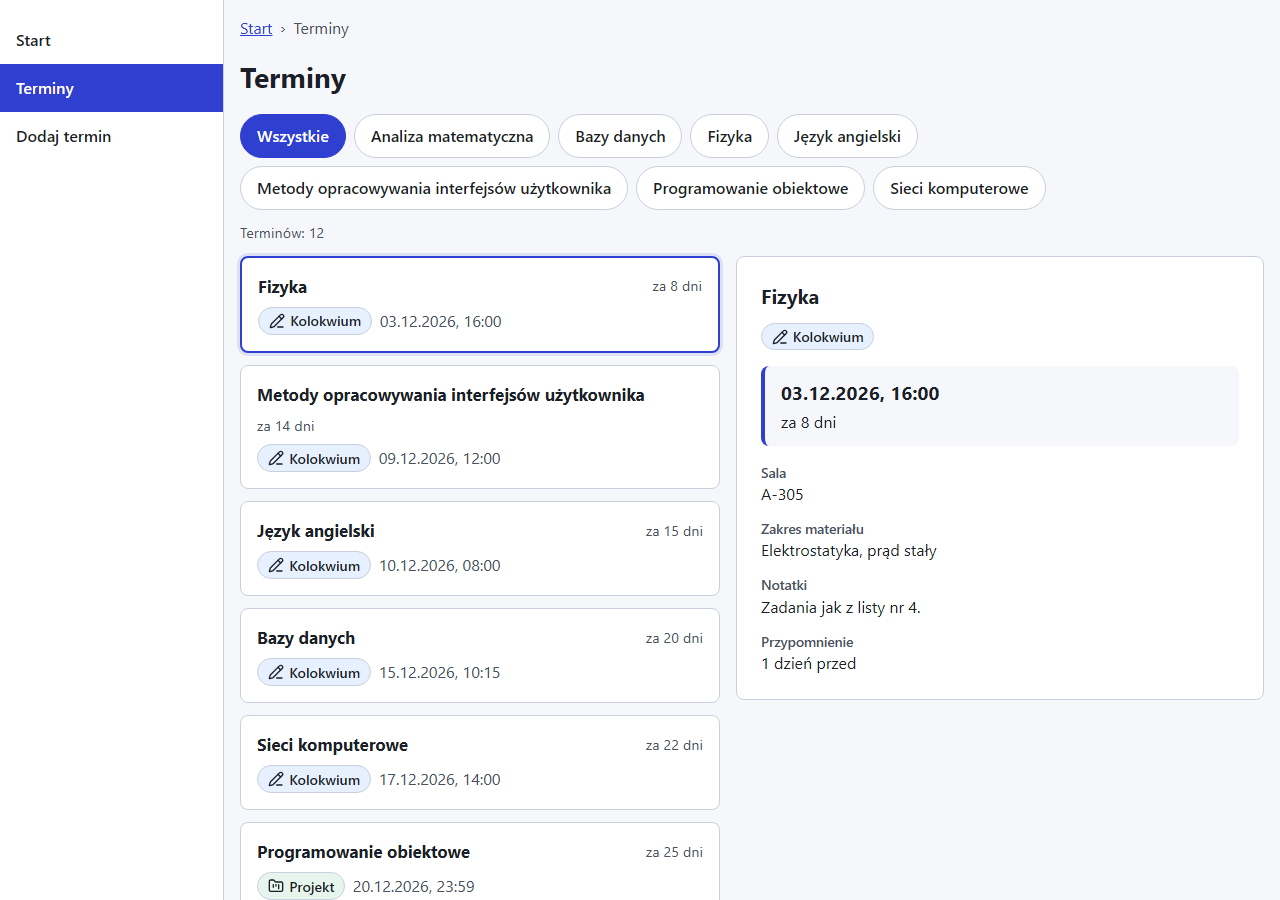
\includegraphics[width=\linewidth]{obrazy/szeroki.png}}{%
  \tikz\node[draw=dkramka,dashed,fill=dkjasny,minimum width=\linewidth,
    minimum height=5.2cm,font=\small\color{dkszary},align=center]{szeroki ekran\\\texttt{obrazy/szeroki.png}};}
\end{minipage}\hfill
\begin{minipage}[b]{0.3\linewidth}\centering
  \IfFileExists{obrazy/waski.png}{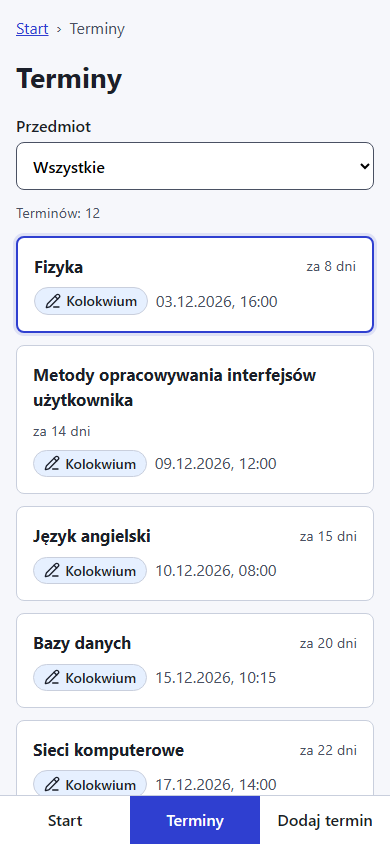
\includegraphics[width=\linewidth]{obrazy/waski.png}}{%
  \tikz\node[draw=dkramka,dashed,fill=dkjasny,minimum width=\linewidth,
    minimum height=5.2cm,font=\small\color{dkszary},align=center]{wąski ekran\\\texttt{obrazy/waski.png}};}
\end{minipage}
\caption{Ten sam ekran w wersji szerokiej i wąskiej}\label{rys:waski}
\end{figure}

% 9. Dostępność
\section{Dostępność}\label{sec:dostepnosc}

\begin{instrukcja}[zalecane]
Kontrast tekstu (co najmniej 4,5:1 dla zwykłego tekstu - Wykład 2), obsługa klawiaturą (Miłość Do Klawiatury
z Wykładu 1: kolejność klawisza Tab, widoczne zaznaczenie), kolor nie jest jedynym nośnikiem informacji (Wykład 3). Wartości kontrastu sprawdźcie
dowolnym narzędziem, np. w narzędziach deweloperskich przeglądarki.
\end{instrukcja}

\begin{table}[H]\centering
\caption{Kontrast par kolorów}\label{tab:kontrast}
\begin{tabularx}{\linewidth}{@{}Lp{2.4cm}p{2.4cm}p{2.2cm}p{2cm}@{}}
\naglowektabeli \nt{Gdzie} & \nt{Tekst} & \nt{Tło} & \nt{Kontrast} & \nt{Wynik} \\
tekst podstawowy na karcie & \#1B1F2A & \#FFFFFF & 16,5:1 & \tak \\
tekst pomocniczy na tle strony & \#4A5163 & \#F6F7FB & 7,4:1 & \tak \\
przycisk główny, aktywne menu & \#FFFFFF & \#2F3FD0 & 7,7:1 & \tak \\
linki i liczba dni & \#2F3FD0 & \#FFFFFF & 7,7:1 & \tak \\
znacznik pilnego terminu & \#B3261E & \#FDECEA & 5,7:1 & \tak \\
\bottomrule
\end{tabularx}
\end{table}

\textbf{Klawiatura:} pierwszy Tab pokazuje odnośnik „Przejdź do treści”, potem menu, okruszki, filtr i kolejne karty w kolejności czytania. Zaznaczenie to niebieska obwódka 3\,px (\texttt{:focus-visible}); na kartach obwódka obejmuje całą kartę. Pełny test klawiaturą zaplanowany na L7.\\
\textbf{Kolor i znaczenie:} typ terminu to ikona i tekst (np. „Kolokwium”), a nie sam kolor tła; termin pilny ma gruby pasek z lewej, ikonę ostrzeżenia i tekst „Za 3 dni”. Animacje (licznik dni, obiegająca ramka) wyłączają się przy ustawieniu systemowym „ogranicz ruch”, a czytnik ekranu dostaje gotową liczbę dni z ukrytego tekstu.

% 10. Samoocena dziesięciu dobrych praktyk
\section{Dziesięć dobrych praktyk - samoocena}\label{sec:samoocena}

\begin{instrukcja}[wymagane]
Dla każdej praktyki z karty projektu wpiszcie \texttt{\textbackslash tak}, \texttt{\textbackslash czesciowo}
albo \texttt{\textbackslash nie} oraz gdzie w projekcie to widać (ekran, element, rozdział). Uczciwa
samoocena jest częścią oceny dokumentacji - „częściowo” z dobrym wyjaśnieniem jest lepsze niż „tak”
bez pokrycia.
\end{instrukcja}

\begin{table}[H]\centering
\caption{Samoocena dziesięciu dobrych praktyk}\label{tab:samoocena}
{\small
\begin{tabularx}{\linewidth}{@{}p{0.5cm}p{4.2cm}p{2.4cm}L@{}}
\naglowektabeli \nt{\#} & \nt{Praktyka} & \nt{Spełniona?} & \nt{Gdzie to widać} \\
1 & Ramy Graficzne & \tak & rozdział \ref{sec:projekt}; wspólny układ i tokeny CSS, menu w tym samym miejscu na każdym ekranie \\
2 & Hierarchia wizualna & \tak & karta najbliższego terminu na Starcie; „Dodaj termin” jedynym wypełnionym przyciskiem \\
3 & Nawigacja i orientacja & \tak & rozdział \ref{sec:nawigacja}; aktywna pozycja menu, okruszki, „Wróć do listy” \\
4 & Lista i szczegóły & \tak & dwa panele na szerokim ekranie, osobny ekran na wąskim (rozdział \ref{sec:waski}) \\
5 & Formularz & \nie & formularz jeszcze w budowie (stan na 25.11) \\
6 & Błędy w formularzu & \nie & reguły w \texttt{validate.ts} gotowe, brak komunikatów przy polach \\
7 & Wartości domyślne i polecenia & \czesciowo & przyciski opisane czasownikami; brak jeszcze formularza i zabezpieczenia usuwania \\
8 & Obsługa klawiaturą & \czesciowo & widoczne zaznaczenie i skip-link; pełny test zaplanowany na L7 \\
9 & Wąski ekran & \tak & jedna kolumna, dolny pasek, cele 48\,px, brak przewijania w bok przy 390\,px \\
10 & Czytelność i dostępność & \tak & rozdział \ref{sec:dostepnosc}; kontrast co najmniej 5,7:1, typ i pilność także tekstem \\
\bottomrule
\end{tabularx}}
\end{table}

% 11. Implementacja
\section{Implementacja}\label{sec:implementacja}

\begin{instrukcja}[zalecane]
Technologie z wersjami, struktura repozytorium i model danych. Nie wklejajcie całego kodu - wystarczą
1-2 najciekawsze fragmenty z krótkim opisem (np. walidacja formularza, zmiana układu na wąskim ekranie).
\end{instrukcja}

\subsection{Technologie}
\begin{table}[H]\centering
\caption{Wykorzystane technologie}\label{tab:technologie}
\begin{tabularx}{\linewidth}{@{}p{3.6cm}p{3.2cm}L@{}}
\naglowektabeli \nt{Technologia} & \nt{Wersja} & \nt{Do czego} \\
Astro & 7.4 & statyczna strona, routing plików, układ \texttt{Layout.astro} \\
React + \texttt{@astrojs/react} & 19.3 / 7.1 & interaktywne wyspy: Start, lista, szczegóły \\
TypeScript & 6.0 & typy danych (\texttt{Termin}) i logika \\
motion & 14.12 & animacja licznika dni (wzór: Magic UI Number Ticker) \\
lucide-react & 1.72 & ikony typów terminów i przycisków \\
CSS (bez frameworka) & -- & tokeny kolorów i odstępów, układ szeroki i wąski \\
\bottomrule
\end{tabularx}
\end{table}

\subsection{Struktura repozytorium}
\noindent\begin{minipage}{\linewidth}
\begin{lstlisting}
MOIU-Planer-Sesji-I-Terminow/
|-- README.md
|-- src/
|   |-- pages/ (index, terminy, termin, dodaj = E1-E4)
|   |-- layouts/Layout.astro (ramy graficzne, menu, skip-link)
|   |-- components/ (Nav, Breadcrumbs, TerminCard, TypBadge,
|   |               ListaTerminow, NajblizszyTermin, SzczegolyTerminu,
|   |               NumberTicker, SpotlightCard)
|   |-- lib/ (store.ts, format.ts, validate.ts, url.ts)
|   |-- data/terminy.json (dane startowe)
|   `-- styles/global.css (tokeny CSS)
`-- docs/ (K1, dokumentacja)
\end{lstlisting}
\end{minipage}

\subsection{Model danych}
Dane startowe są w \texttt{src/data/terminy.json} (12 terminów). Przy pierwszym wejściu aplikacja kopiuje je do \texttt{localStorage} i dalej wszystkie operacje działają tam (\texttt{store.ts}). Przykładowy rekord:
\begin{lstlisting}[language=json]
{
  "id": "t3",
  "przedmiot": "Metody opracowywania interfejsow uzytkownika",
  "typ": "kolokwium",
  "data": "2026-12-09",
  "godzina": "12:00",
  "sala": "B-204",
  "zakres": "Wyklady 1-4",
  "notatki": "",
  "przypomnienie": "1d"
}
\end{lstlisting}

\subsection{Wybrany fragment kodu}
Na liście ten sam link zachowuje się różnie zależnie od szerokości ekranu (\texttt{TerminCard.tsx}):
\begin{lstlisting}
function klik(e) {
  if (onWybierz && matchMedia('(min-width: 48rem)').matches) {
    e.preventDefault();   // szeroki ekran: zostajemy na liscie
    onWybierz(t.id);      // i pokazujemy szczegoly w panelu obok
  }                       // waski ekran: zwykle przejscie do /termin?id=
}
\end{lstlisting}
Karta jest zwykłym odnośnikiem, więc działa bez JavaScriptu, z klawiatury i w nowej karcie przeglądarki.
Tylko na szerokim ekranie kliknięcie jest przechwytywane i zmienia panel szczegółów oraz adres strony
(\texttt{history.replaceState}).

% 12. Instrukcja uruchomienia
\section{Instrukcja uruchomienia}\label{sec:uruchomienie}

\begin{instrukcja}[wymagane]
Krok po kroku, tak żeby prowadząca mogła uruchomić projekt na swoim komputerze: co zainstalować, jakie
polecenia wydać, gdzie otworzyć aplikację. Sprawdźcie instrukcję na komputerze osoby, która nie
pisała kodu.
\end{instrukcja}

\begin{ramka}{Szybki start}
\textbf{Repozytorium:} \dkpokaz{repozytorium}\\
\textbf{Dane testowe:} aplikacja startuje z 12 przykładowymi terminami; konto nie jest potrzebne. Żeby wrócić do danych startowych, wystarczy usunąć klucz \texttt{planer-sesji:terminy} z \texttt{localStorage}.
\end{ramka}

\subsection{Wymagania}
\begin{itemize}
  \item Node.js 22.23.4 lub nowszy (z npm), Git
  \item przeglądarka: Chrome, Firefox albo Edge
\end{itemize}

\subsection{Uruchomienie lokalne}
\noindent\begin{minipage}{\linewidth}
\begin{lstlisting}[style=konsola]
git clone https://github.com/Machux133/MOIU-Planer-Sesji-I-Terminow.git
cd MOIU-Planer-Sesji-I-Terminow
npm install
npm run dev
# adres: http://localhost:4321/MOIU-Planer-Sesji-I-Terminow/
\end{lstlisting}
\end{minipage}

% 13. Testy
\section{Testy i znane ograniczenia}\label{sec:testy}

\begin{instrukcja}[zalecane]
Jak sprawdziliście, że aplikacja działa: scenariusze testowe powiązane z wymaganiami (rozdział
\ref{sec:wymagania}), urządzenia i przeglądarki. Uczciwie wypiszcie znane błędy i ograniczenia.
\end{instrukcja}

\begin{table}[H]\centering
\caption{Scenariusze testowe}\label{tab:testy}
{\small
\begin{tabularx}{\linewidth}{@{}p{1.1cm}p{1.4cm}LLp{1.6cm}@{}}
\naglowektabeli \nt{ID} & \nt{Wymag.} & \nt{Kroki} & \nt{Oczekiwany wynik} & \nt{Wynik} \\
T-1 & WF-3 & \wpisz{otwórz formularz, zostaw puste pole tytułu, zapisz} & \wpisz{komunikat przy polu, pozostałe dane zostają} & \wpisz{\tak} \\
T-2 & WN-1 & \wpisz{zwęź okno do 360 px} & \wpisz{brak przewijania w bok} & \\
T-3 & \wpisz{...} & & & \\
\bottomrule
\end{tabularx}}
\end{table}

\textbf{Testowane na:} \wpisz{urządzenia, systemy, przeglądarki.}

\subsection{Znane błędy i ograniczenia}
\begin{itemize}
  \item \wpisz{np. brak trybu offline}
  \item \wpisz{...}
\end{itemize}

% 14. Organizacja pracy
\section{Organizacja pracy}\label{sec:organizacja}

\begin{instrukcja}[wymagane]
Kto za co odpowiadał i jak pracowaliście. Każda osoba musi umieć wyjaśnić dowolny fragment kodu -
także ten, którego nie pisała. Przy narzędziach AI napiszcie konkretnie, do czego ich używaliście
i czego nie robiły za Was.
\end{instrukcja}

\subsection{Podział pracy}
\begin{table}[H]\centering
\caption{Podział pracy w zespole}\label{tab:podzial}
\begin{tabularx}{\linewidth}{@{}p{4.4cm}Lp{2cm}@{}}
\naglowektabeli \nt{Osoba} & \nt{Za co odpowiadała} & \nt{Udział} \\
Mateusz Machowski & ramy graficzne, nawigacja, ekrany E1-E3, wąski ekran; rozdziały 4, 5, 8 & \wpisz{50\%} \\
Bartosz Kurbiel & repozytorium, formularz E4, walidacja, dane i operacje; rozdziały 7, 9 & \wpisz{50\%} \\
\bottomrule
\end{tabularx}
\end{table}

\subsection{Sposób pracy}
Zadania podzieliliśmy według terminów z harmonogramu w pliku \texttt{docs/PODZIAL\_PRACY.md}: osoba A
odpowiada za ramy, start, listę i szczegóły, osoba B za formularz, dane i operacje. Kod jest w jednym
repozytorium na GitHubie; każdą zmianę ogląda druga osoba.

\subsection{Wykorzystanie narzędzi AI}
\begin{tabularx}{\linewidth}{@{}p{3.6cm}p{3.2cm}L@{}}
\naglowektabeli \nt{Narzędzie} & \nt{Kto używał} & \nt{Do czego} \\
Claude Code (Anthropic) & M. Machowski & szkic komponentów listy, karty i szczegółów, efektów wizualnych (licznik dni, podświetlenie kart), zrzuty ekranu i pierwsza wersja tekstu dokumentacji \\
\wpisz{...} & & \\
\bottomrule
\end{tabularx}

\medskip
Decyzje projektowe (model nawigacji, wybór wzorców, zakres) podjęliśmy sami na podstawie wykładów
i makiet z K1. Wygenerowany kod przeglądaliśmy i uruchamialiśmy na szerokim i wąskim ekranie; podczas
sprawdzania zrzutów wyszły dwa błędy na telefonie (pasek menu przykryty przez karty, za szerokie pole
wyboru), które poprawiliśmy. Każda osoba potrafi wyjaśnić kod obu części.

% 15. Podsumowanie
\section{Podsumowanie}\label{sec:podsumowanie}

\begin{instrukcja}[zalecane]
Krótka refleksja: co się udało, co było trudne, co poprawilibyście w kolejnej wersji i czego
nauczyliście się o projektowaniu interfejsów. Pół strony.
\end{instrukcja}

\subsection{Co się udało}
\wpisz{...}

\subsection{Co poprawilibyśmy}
\wpisz{...}

\subsection{Wnioski}
\wpisz{...}

% 16. Źródła i licencje
\section{Źródła i licencje}\label{sec:zrodla}

\begin{instrukcja}[wymagane]
Skąd pochodzą zdjęcia, ikony, fonty, biblioteki i gotowe fragmenty kodu, na jakiej licencji. Jeśli
wszystko jest własne - napiszcie to. Literaturę podajcie w formie listy.
\end{instrukcja}

\subsection{Materiały i biblioteki}
\begin{table}[H]\centering
\caption{Wykorzystane materiały i ich licencje}\label{tab:licencje}
{\small
\begin{tabularx}{\linewidth}{@{}p{3cm}p{3.4cm}p{2.6cm}L@{}}
\naglowektabeli \nt{Zasób} & \nt{Nazwa} & \nt{Licencja} & \nt{Źródło} \\
ikony & Lucide (\texttt{lucide-react}) & ISC & \url{https://lucide.dev} \\
font & systemowy (Segoe UI, Roboto) & -- & nie pobieramy fontów \\
zdjęcia & brak & -- & -- \\
efekty & wzory: Magic UI (Number Ticker, Border Beam), React Bits (Spotlight Card) & MIT & \url{https://magicui.design}, \url{https://reactbits.dev}; kod napisany od nowa \\
biblioteki & Astro, React, motion & MIT & \url{https://astro.build}, \url{https://react.dev}, \url{https://motion.dev} \\
\bottomrule
\end{tabularx}}
\end{table}

\subsection{Literatura}
\begin{enumerate}[label={[\arabic*]}]
  \item J. Tidwell, \emph{Projektowanie interfejsów. Sprawdzone wzorce projektowe}, wyd. II, Helion, 2020.
  \item Prezentacje z wykładów 1-4, Metody opracowywania interfejsów użytkownika, UKEN 2026/27.
  \item Dokumentacja Astro, \url{https://docs.astro.build}; dokumentacja React, \url{https://react.dev}.
\end{enumerate}


% załączniki
\appendix
% Załączniki
\section{Makiety z punktu kontrolnego K1}\label{zal:makiety}

\begin{instrukcja}[zalecane]
Makiety low-fi oddane jako K1 (mogą być zdjęcia rysunków odręcznych). Dzięki nim widać, jak projekt
się zmieniał.
\end{instrukcja}

\zrzut{mapa_ekranow.png}{Mapa ekranów z K1}{0.9}
\zrzut{makieta_lista.png}{Makieta z K1: lista terminów na komputerze}{0.8}
\zrzut{makieta_formularz.png}{Makieta z K1: formularz po próbie zapisu bez daty}{0.5}
\zrzut{makieta_telefon.png}{Makieta z K1: ekran startowy na telefonie}{0.35}

\section{Zrzuty wszystkich ekranów}\label{zal:ekrany}
\zrzut{e1_start.png}{E1 - ekran startowy}{0.75}
\zrzut{e1_start_waski.png}{E1 - ekran startowy na telefonie}{0.35}
\zrzut{e2_lista.png}{E2 - lista}{0.75}
\zrzut{e3_szczegoly.png}{E3 - szczegóły na telefonie}{0.35}
\zrzut{e4_formularz.png}{E4 - formularz (w budowie)}{0.75}


\end{document}
